\documentclass[11pt,letterpaper]{article}
\usepackage[top=3cm, bottom=2cm, left=2cm, right=2cm, columnsep=20pt]{geometry}
\usepackage{pdfpages}
\usepackage{graphicx}
\usepackage{etoolbox}
\apptocmd{\sloppy}{\hbadness 10000\relax}{}{}
 \usepackage[numbers]{natbib}
\usepackage[T1]{fontenc}
\usepackage{ragged2e}
\usepackage[french]{babel}
\usepackage{listings}
\usepackage{color}
\usepackage{soul}
\usepackage[utf8]{inputenc}
\usepackage[export]{adjustbox}
\usepackage{caption}
\usepackage{amsmath}
\usepackage{amssymb}
\usepackage{float}
\usepackage{csquotes}
\usepackage{fancyhdr}
\usepackage{wallpaper}
\usepackage{siunitx}
\usepackage[indent]{parskip}
\usepackage{textcomp}
\usepackage{gensymb}
\usepackage{multirow}
\usepackage[hidelinks]{hyperref}
\usepackage{abstract}
\renewcommand{\abstractnamefont}{\normalfont\bfseries}
\renewcommand{\abstracttextfont}{\normalfont\itshape}
\usepackage{titlesec}
\titleformat{\section}{\large\bfseries}{\thesection}{1em}{}
\titleformat{\subsection}{\normalsize\bfseries}{\thesubsection}{1em}{}
\titleformat{\subsubsection}{\normalsize\bfseries}{\thesubsubsection}{1em}{}

\usepackage{xcolor}
\definecolor{codegreen}{rgb}{0,0.6,0}
\definecolor{codegray}{rgb}{0.5,0.5,0.5}
\definecolor{codepurple}{rgb}{0.58,0,0.82}
\definecolor{backcolour}{rgb}{0.95,0.95,0.92}
\lstdefinestyle{mystyle}{
    backgroundcolor=\color{backcolour},   
    commentstyle=\color{codegreen},
    keywordstyle=\color{magenta},
    numberstyle=\tiny\color{codegray},
    stringstyle=\color{codepurple},
    basicstyle=\ttfamily\footnotesize,
    breakatwhitespace=false,         
    breaklines=true,                 
    captionpos=b,                    
    keepspaces=true,                 
    numbers=left,                    
    numbersep=5pt,                  
    showspaces=false,                
    showstringspaces=false,
    showtabs=false,                  
    tabsize=2
}
\lstset{style=mystyle}

\usepackage[most]{tcolorbox}
\newtcolorbox{note}[1][]{
  enhanced jigsaw,
  borderline west={2pt}{0pt}{black},
  sharp corners,
  boxrule=0pt, 
  fonttitle={\large\bfseries},
  coltitle={black},
  title={Note:\ },
  attach title to upper,
  #1
}

%----------------------------------------------------

\setlength{\parindent}{0pt}
\DeclareCaptionLabelFormat{mycaptionlabel}{#1 #2}
\captionsetup[figure]{labelsep=colon}
\captionsetup{labelformat=mycaptionlabel}
\captionsetup[figure]{name={Figure }}
\newcommand{\inlinecode}{\normalfont\texttt}
\usepackage{enumitem}
\setlist[itemize]{label=\textbullet}

\begin{document}
\begin{titlepage}
\center

\begin{figure}
    \ThisULCornerWallPaper{.4}{Polytechnique_signature-RGB-gauche_FR.png}
\end{figure}
\vspace*{2 cm}

\textsc{\Large \textbf{PHS2223 --} Introduction à l'optique moderne}\\[0.5cm]
\large{\textbf{Équipe : 04}}\\[1.5cm]

\rule{\linewidth}{0.5mm} \\[0.5cm]
\Large{\textbf{Expérience 2}} \\[0.2cm]
\text{Objectif de caméra}\\
\rule{\linewidth}{0.2mm} \\[2.3cm]

\large{\textbf{Présenté à}\\
  Guillaume Sheehy\\
  Esmat Zamani\\[2.5cm]
  \textbf{Par :}\\
  Émile \textbf{Guertin-Picard} (2208363)\\
  Laura-Li \textbf{Gilbert} (2204234)\\
  Tom \textbf{Dessauvages} (2133573)\\[3cm]}

\large{\today\\
Département de Génie Physique\\
Polytechnique Montréal\\}

\end{titlepage}

%----------------------------------------------------

\tableofcontents
\pagenumbering{roman}
\newpage

\pagestyle{fancy}
\setlength{\headheight}{14pt}
\renewcommand{\headrulewidth}{0pt}
\fancyfoot[R]{\thepage}

\pagestyle{fancy}
\fancyhf{}
\renewcommand{\headrulewidth}{1pt}
\fancyhead[L]{\textbf{PHS2223}}
\fancyhead[C]{Rapport préliminaire}
\fancyhead[R]{\today}
\fancyfoot[R]{\thepage}

\pagenumbering{arabic}
\setcounter{page}{1}

%----------------------------------------------------

\section{Introduction}

Les objectifs de caméras modernes sont des systèmes physiques complexes, permettant de définir l'identité d'une image et dépendent, par conséquent, de la façon dont l'observateur veut représenter l'objet d'intérêt. Dans le cas le plus simple possible, soit le cas d'étude de ce laboratoire, ces objectifs sont constitués de trois lentilles : une fixe, permettant de former une image nette, et deux mobiles, utiles à l'ajustement de paramètres d'observations. Le premier de ces paramètres est lié au grossissement de l'objet observé. Pour prendre une photo ou filmer une image lointaine, il faudra, par exemple, opter pour un téléobjectif à fort grossissement, ce qui n'est pas le cas lorsque le but est de faire un portrait rapproché. Cependant, décoller un portrait de l'arrière plan permet souvent de le mettre en valeur en le faisant ressortir. Ce flou recherché derrière l'objet observé est lié au deuxième paramètre étudié, appelé la profondeur de champ. Elle détermine le facteur de netteté associé à un éloignement vis-à-vis du point focal. Une grande profondeur de champ permettra donc de détailler l'arrière plan tandis qu'une faible profondeur de champ le flouera. Un dernier paramètre, davantage lié au système optique complet de l'objectif et de la mise en relation de ses éléments, nommé vignettage, définit l'assombrissement des bords de l'image en raison de l'ouverture d'arrêt. Le but de ce laboratoire est donc de caractériser un objectif de caméra simple, composé de trois lentilles. Les attentes sont de se familiariser et comprendre l'impact des paramètres d'observation de l'objectif sur une image enregistrée, tout en continuant de développer des habilités liée à l'alignement de systèmes optiques. Le présent rapport, présente la préparation à ce laboratoire, de la compréhension théorique du système étudié, à la méthodologie prévue pour ses manipulations ainsi que les hypothèses émises quant à leurs résultats. 

\section{Théorie}

\subsection{Grossissement}
Le grossissement correspond à l'augmentation apparente de la taille d'un objet lorsque celui-ci est observé à travers un système optique. En termes techniques, il s'agit d'un rapport entre la taille apparente de l'image et celle réelle \cite{blondeau_grossissement_2023}.

Avec le grossissement, il est possible de déterminer le facteur de zoom. Ce facteur, offrant une description de l'agrandissement ou de la réduction des images, est le ratio entre le grossissement maximal et le grossissement minimal obtenu \cite{noauthor_videoprojecteur_2024}.

\subsection{Profondeur de champ}
La profondeur de champ décrit la distance autour du plan de mise au point avec laquelle les objets apparaissent suffisamment nets. En d'autres termes, ce concept optique réfère à la distance entre les points les plus rapprochés et ceux les plus éloignés du sujet qui sont reproduits avec une netteté acceptable dans une image \cite{hollows_depth_2023}. Appliquée à plusieurs sytèmes optiques tels que les caméras et les microscopes, cette notion de profondeur est influencée par les paramètres suivants : la distance focale, l'ouverture de l'objectif, et la distance de l'objet \cite{leblond_semaine_2024}. 

\subsection{Vignettage}
Le vignettage, phénomène photographique, correspond à une diminution de la lumiosité vers les périphéries de l'image. Ce phénomène peut résulter de la conception optique, soit l'ajout d'une ouverture d'arrêt afin de limiter la lumière entrante, une obstruction, ou encore, la focalisation \cite{cognard_comprendre_2017}.

\subsection{Résolution}
La résolution, pour un système optique, correspond à la capacité de reproduire les détails d'une image, c'est-à-dire la distance minimale à laquelle deux points sur l'axe optique peuvent être distingués \cite{fouquet_improving_2015}, tels que la longueur d'onde, l'ouverture d'arrêt, et le système lui-même \cite{jonkman_18_2003}. Ici, c'est donc la taille d'un pixel de caméra dans l'espace objet.

\subsection{Lentilles optiques}
Les lentilles optiques se catégorisent en quelques types, notamment les lentilles convergentes et les divergentes. Celles-ci ont pour fonction de concentrer ou de disperser les rayons traversant un système à l'aide du principe de réfraction. Dans le cas des lentilles convergentes, celles-ci permettent à des faisceaux parallèles de converger en un point spécifique de l'axe optique, soit le point focal \cite{noauthor_thin_nodate}, nommée la distance focale. 

Les lentilles divergentes, pour leur part, permettent de disperser les faisceaux, et de ne former qu'une tâche lumineuse. Contrairement aux lentilles convergentes, le point focal des lentilles divergentes se situent dans l'espace image et correspond au prolongement des rayons divergents \cite{zimmermann_lentilles_2015}. 

\subsection{Méthode des matrices}
La méthode des matrices, également connue sous le nom d'optique matricielle, est une technique de résolution utilisée en optique complexe. Cette méthode permet d'étudier le comportement des faisceaux à travers un système optique à l'aide de l'algèbre linéaire. De cette manière, cette technique repose sur les relations linéaires entre les grandeurs entrantes et sortantes, permettant d'utiliser une matrice (2$\times$2) pour exprimer les transformations subies par ces grandeurs. Lorsqu'un rayon traverse un système optique, tel qu'illustré dans la figure ci-dessous, celui-ci est caractérisé par des paramètres d'entrée, soient un angle $\theta_1$ et une hauteur $x_1$, ainsi que des paramètres de sortie, soient un angle $\theta_2$ et une hauteur $x_2$.
\begin{figure}[H]
  \centering
  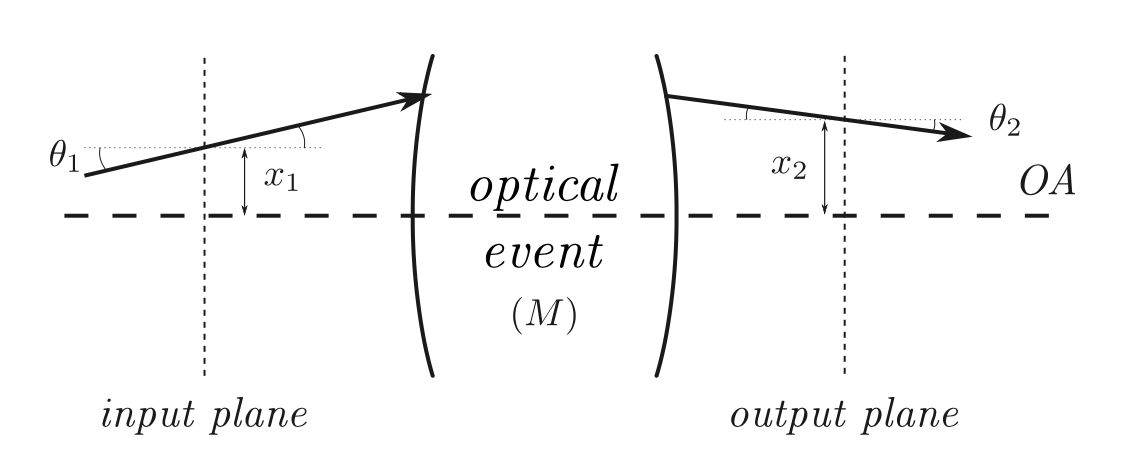
\includegraphics[scale=0.5]{methode_math.png}
  \caption{Schéma d'un transfert de rayon dans un système optique.}
  \label{methode_math}
\end{figure}
Avec ces schémas optiques, il est possible de définir, pour chaque élément du système en question, une matrice de la forme suivante :
\begin{gather}
  \begin{pmatrix}
    x_2 \\
    \theta_2 \\
  \end{pmatrix}=
  \begin{pmatrix}
    A & B \\
    C & D \\
  \end{pmatrix}
  \begin{pmatrix}
    x_1 \\
    \theta_1 \\
  \end{pmatrix}
\end{gather}
Ainsi, en fonction des différentes composantes du système optique, telles qu'une lentille, un miroir ou un milieu de propagation, la matrice, illustée à l'équation (2), prend les formes appropriées \cite{leblond_semaine_2024-1}.


\subsection{Système de caméra}

La figure \ref{schema_syst}, tirée de l'énoncé du laboratoire \cite{sheehy_experience_2024}, présente
l'intérieur du système de caméra sous forme de schéma des lentilles :

\begin{figure}[H]
  \centering
  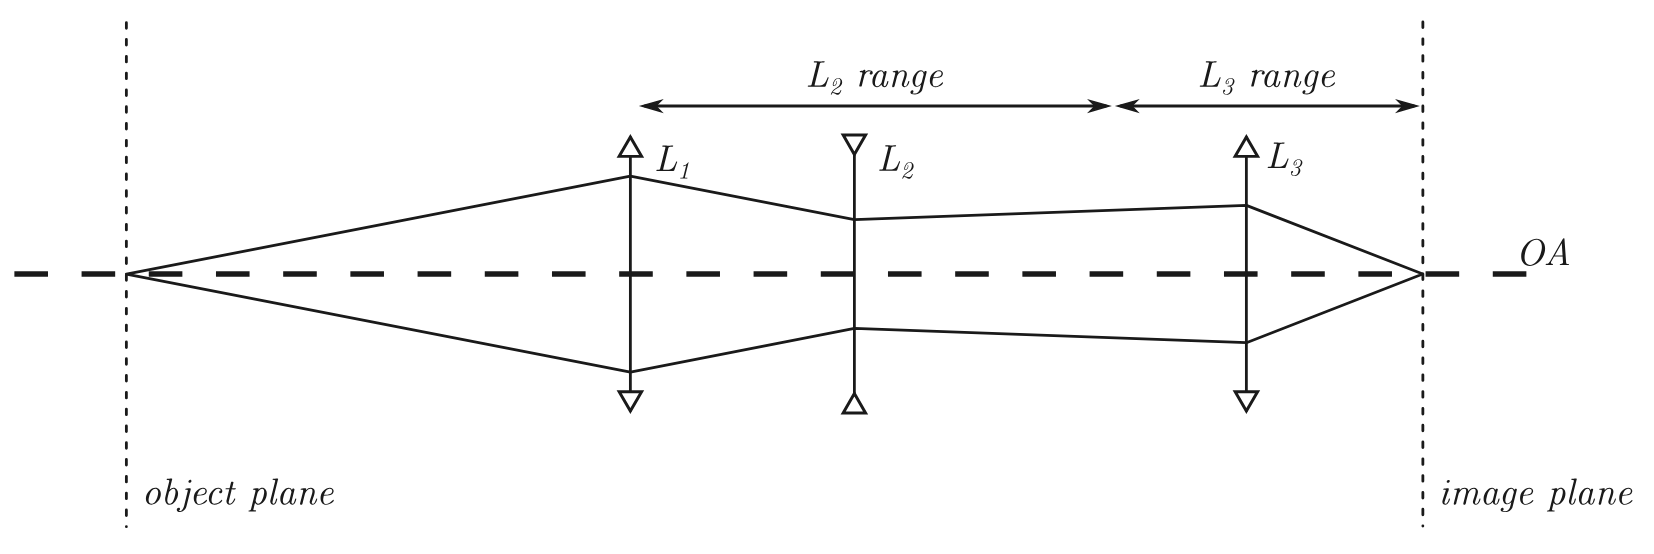
\includegraphics[scale=0.2]{systeme_optique.png}
  \caption{Schéma du système optique d'objectif de caméra à zoom et focus ajustable}
  \label{schema_syst}
\end{figure}

Ce schéma présente le parcours des faisceaux à travers l'objectif d'une caméra à focus ajustable. De ce fait, il est possible d'observer que le rayon se propage, d'abord, dans la caméra, puis rencontre une première lentille. Cette lentille ($L_1$) convergente permet aux rayons de se diriger vers une seconde lentille ($L_2$) qui, pour sa part, provoque la divergence de ces rayons. Après avoir traversé cette seconde lentille, ceux-ci se dirige vers une troisième et dernière lentille ($L_3$), convergeant les faisceaux en un point afin de former l'image finale. La maniabilité des lentilles $L_2$ et $L_3$ permettent d'ajuster les facteurs de grossissement et de focus de la caméra. Ainsi, à partir de la figure ci-dessus, la méthode des matrices, expliquée à la section 2.4, est appliquée afin de caractériser le système et de déterminer ces dits facteurs.


\subsection{Modélisation mathématique par matrice de transfert}
À l'aide de la figure \ref{schema_syst}, représentant visuellement les rayons à travers le système optique, il est possible de poser une matrice de transfert $M$ de la manière suivante :
\begin{equation}
  M=M_{T7}M_{F6}M_{T5}M_{F4}M_{T3}M_{F2}M_{T1}
\end{equation}
Chacune de ces matrices représentent une composante du système optique. Ces composantes sont les suivantes :
\begin{itemize}
  \item $M_{T1}$ est une matrice de translation de la distance entre le plan objet et la lentille $L_1$
  \item $M_{F2}$ est une matrice de lentille mince pour la lentille $L_1$
  \item $M_{T3}$ est une matrice de translation de la distance entre les lentilles $L_1$ et $L_2$
  \item $M_{F4}$ est une matrice de lentille mince pour la lentille $L_2$
  \item $M_{T5}$ est une matrice de translation de la distance entre les lentilles $L_2$ et $L_3$
  \item $M_{F6}$ est une matrice de lentille mince pour la lentille $L_3$
  \item $M_{T7}$ est une matrice de translation de la distance entre la lentille $L_3$ et le plan image
\end{itemize}
La forme des matrices de translation est donnée par :
\begin{gather}
  M_T=
  \begin{bmatrix}
    1 & d \\
    0 & 1 \\
  \end{bmatrix}
\end{gather}
Où $d$ correspond à la longueur de la translation selon l'axe optique, soit la distance entre deux points données. Les matrices de lentille mince sont définies par la forme suivante :
\begin{gather}
  M_T=
  \begin{bmatrix}
    1 & 0 \\
    -\frac{1}{f} & 1 \\
  \end{bmatrix}
\end{gather}
Où $f$ est la distance focale de la lentille. Les rayons traversant ces matrices sont caractérisés, tel mentionné dans la section 2.4, par certains paramètres soient les angles et les hauteurs entrantes et sortantes. Ceux-ci sont utiles à la paramétrisation de la distance entre les lentilles. Pour ce faire, un rayon initial $r_i$ à une hauteur $y_i$, soit nulle, et un angle $\alpha_i$, quelconque, partant du plan objet, et un rayon final $r_f$ à une hauteur $y_f$, aussi nulle, et un angle $\alpha_f$ sont considérés. Ces faisceaux permettent la formation de l'équation suivante :
\begin{gather}
  \begin{bmatrix}
    0 \\
    \alpha_f \\
  \end{bmatrix}=M
  \begin{bmatrix}
    0 \\
    \alpha_i \\
  \end{bmatrix}
\end{gather}
Les hauteurs $y_i$ et $y_f$ sont nulles puisque les rayons de lumière commencent à un certain point sur l'axe optique et se termine à un autre point sur l'axe optique. En résolvant ce système matriciel, deux solutions, sous forme de racine, sont obtenues. Afin de déterminer laquelle de ces solutions est celle désirée, elles sont vérifiées à l'aide des différentes distances possibles entre les lentilles. De cette manière, en calculant les solutions avec les positionnements extrêmes de la seconde lentille $L_2$, soit à la distance minimale et maximale, la solution offrant une racine position et réelle est considérée comme la paramétrisation optimale.

\subsubsection{Paramétrisation du grossissement}
La matrice de transfert $M$, définie à l'aide de la modélisation mathématique précédente, est notée de la manière suivante :
\begin{gather}
  M=
  \begin{bmatrix}
    A & B \\
    C & D \\
  \end{bmatrix}
\end{gather}
À partir de cette notation, il est possible de déterminer le grossissement d'un système, correspondant à la valeur de $A$. De cette manière, la paramétrisation du grossissement en fonction de la distance entre les lentilles peut être visualisée.

\section{Méthodologie}

La méthode utilisée pour ce laboratoire vise à caractériser un objectif de caméra simple, composé de trois lentilles. La figure \ref{montage} présente sous la forme d'un schéma et d'une photographie, le montage utilisé ainsi que son système optique. 

\begin{figure}[H]
  \centering
  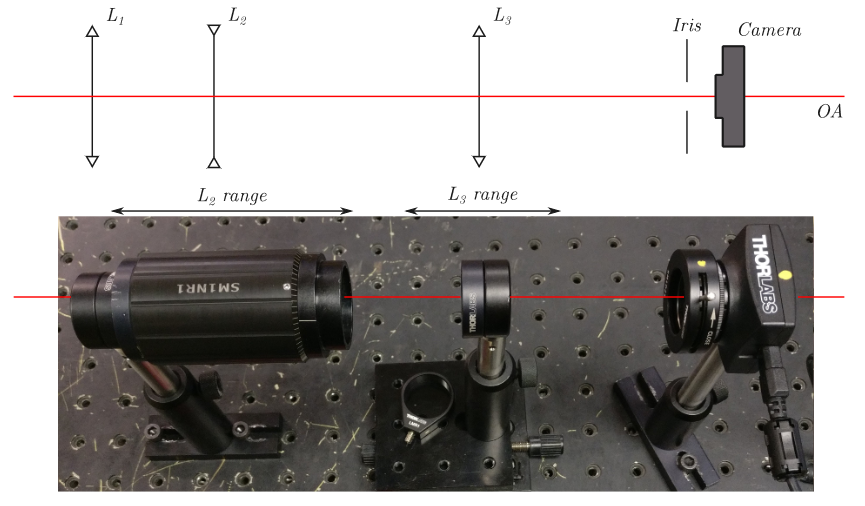
\includegraphics[scale=0.45]{Montage laboratoire 2.png}
  \caption{Schéma du système optique (en haut) du montage (en bas) utilisé pour le laboratoire.}
  \label{montage}
\end{figure}

Le matériel utilisé pour ce montage est le suivant : 

\begin{itemize}
    \item Lentille $L_1 = 150 mm$, $\phi_1 = 25.4 mm$
    \item Lentille $L_2 = -75 mm$, $\phi_1 = 25.4 mm$
    \item Lentille $L_3 = 75 mm$, $\phi_1 = 25.4 mm$
    \item Iris ajustable SM1D25
    \item Tube à lentille ajustable 75 mm (\textit{zoom housing}) SM1NR1
    \item Plateforme de translation > 25 mm
    \item Caméra USB Thorlabs DDC1645C
    \item Pièces optomécaniques nécessaires (BA1, PH2, PH3, TR2, TR3, LMR1, ...)
\end{itemize}

La première étape consiste à aligner le montage, en utilisant des iris d'alignement et en maximisant le focus sur la caméra. Il faudra ensuite, pour chaque paramètre, établir une série de mesures en fonction de la variable d'intérêt. La liste des clichés à prendre est : 

\begin{itemize}
    \item La profondeur de champ à 1 m (2 positions extrêmes du zoom)
    \item La résolution à 1 m (2 positions extrêmes du zoom)
    \item Mesure du vignetting à 1 m et à $\infty$ (2 positions extrêmes du zoom)
    \item Image d’objet à l’infini (2 positions extrêmes du zoom)
\end{itemize}

Dans tous les cas, les clichés seront à prendre en double, pour chacune des valeurs extrêmes de zoom. La lentille $L_2$ sera donc toujours placée aux extrémités de sa plage de déplacement. Pour ce qui est de $L_3$, elle sera positionnée de sorte que l'objet d'intérêt soit toujours au focus. L'objet imagé sera positionné en fonction du paramètre à mesurer, soit à un mètre pour le grossissement et la résolution, et à un mètre puis l'infini pour le vignettage. Dans le cas de la profondeur de champ, puisqu'elle nécessite de mesurer une plage de valeur, l'objet sera positionné à un mètre de l'objectif, puis avancé et ensuite reculé jusqu'à sortir du plan focal, afin de déterminer la distance entre les valeurs d'avancement et d'éloignement maximum.

\section{Hypothèses}

Afin de pouvoir prédire les phénomènes qui pourront être observés en laboratoire, un
programme Python a été développé afin de résoudre analytiquement
le système par la méthode des matrices. Ce programme commence tout d'abord par construire
la matrice de transfert du système, puis il paramétrise l'écart entre les lentilles selon
la position de $L_2$ par rapport à $L_1$. Enfin, il calcule les différentes caractéristiques
qui suivent.

\subsection{Profondeur de champ}

Premièrement, le programme calcule la profondeur de champ en fonction de la position de
la lentille $L_2$. Le résultat est présenté à la figure \ref{prof_champ_plot}.

\begin{figure}[H]
  \centering
  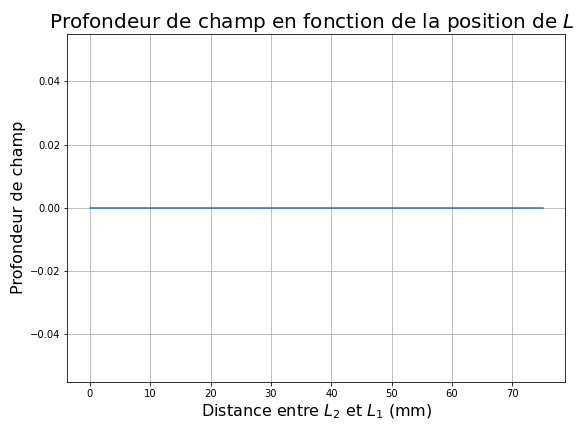
\includegraphics[scale=0.55]{prof_champ.png}
  \caption{Graphique de la profondeur de champ en fonction de la position de la lentille 
  $L_2$ suite au calcul de Python}
  \label{prof_champ_plot}
\end{figure}

Ainsi, il est possible de faire comme hypothèse que la profondeur du champ n'est pas affectée
par la position de $L_2$.

\subsection{Résolution}

Ensuite, la figure \ref{gross_plot} montre le grossissement de l'image en fonction de la
position de $L_2$.

\begin{figure}[H]
  \centering
  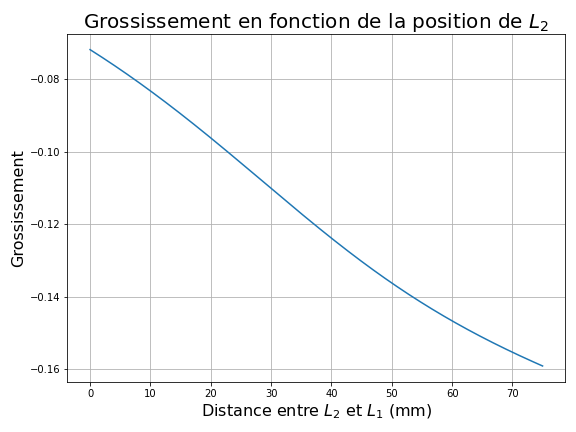
\includegraphics[scale=0.55]{grossissement.png}
  \caption{Graphique du grossissement d'une image en fonction de la position de la lentille
  $L_2$ suite au calcul de Python.}
  \label{gross_plot}
\end{figure}

Découlant directement de ce résultat, il est possible de visualiser la résolution en fonction
de la position de la lentille, tel que montré à la figure \ref{res_plot}. Cela montre la taille
d'un pixel de la caméra (\textit{pixel pitch}), qui vaut 3.6 micromètres pour la caméra THORLABS, dans le plan objet \cite{thorlabs}.

% Source B : https://www.thorlabs.com/catalogpages/obsolete/2020/DCC1645C.pdf

\begin{figure}[H]
  \centering
  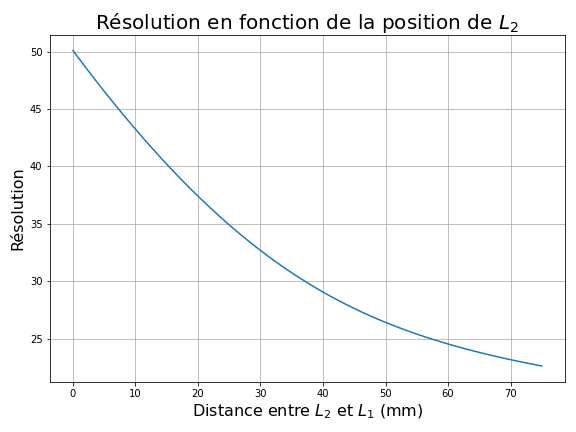
\includegraphics[scale=0.55]{Resolution.png}
  \caption{Graphique de la résolution de la caméra en fonction de la position de la lentille
  $L_2$ suite au calcul de Python.}
  \label{res_plot}
\end{figure}

Ainsi, il est possible de prédire que le grossissement (qui est inversé en raison du signe 
négatif) augmente plus la distance entre $L_2$ et $L_1$ augmente. Sans surprise, une relation 
réciproque est prédite pour la résolution, qui décroît plus cette distance augmente.

\subsection{Facteur de zoom}

Enfin, selon la figure \ref{gross_plot}, il est possible de prendre les deux extrêmes de la courbe 
pour trouver une prédiction dufacteur de zoom. Calculé par le programme, le résultat est un facteur
d'environ 0.45.
\clearpage

\bibliographystyle{unsrtnat}
\bibliography{camera_prelab.bib}

\end{document}
